%
% $RCSfile: synchronous_execution.tex,v $
%
% Copyright (c) 2002-2007. Christian Heller. All rights reserved.
%
% Permission is granted to copy, distribute and/or modify this document
% under the terms of the GNU Free Documentation License, Version 1.1 or
% any later version published by the Free Software Foundation; with no
% Invariant Sections, with no Front-Cover Texts and with no Back-Cover
% Texts. A copy of the license is included in the section entitled
% "GNU Free Documentation License".
%
% http://www.cybop.net
% - Cybernetics Oriented Programming -
%
% Version: $Revision: 1.1 $ $Date: 2007-08-01 13:59:00 $ $Author: christian $
% Authors: Christian Heller <christian.heller@tuxtax.de>
%

\subsection{Synchronous Execution}
\label{synchronous_execution_heading}
\index{Synchronous Execution Example}
\index{MusicXML}

\emph{MusicXML} \cite{musicxml} is a markup language \textit{designed to
represent musical scores, specifically common western musical notation from the
17th century onwards.} In principle, CYBOL could be used for this purpose as
well. Of course, there are many details (additional properties) which would
still have to be worked out in order to be able to correctly represent complete
musical scores. As most models, the \emph{Musical Work} displayed in figure
\ref{music_figure} can be considered a hierarchy consisting of \emph{Parts}
(played/ sung by instruments/ voices). Parts in turn consist of
\emph{Measures}, which consist of \emph{Notes}, which finally have a
\emph{Pitch} and sometimes \emph{Lyric}.

\begin{figure}[ht]
    \begin{center}
        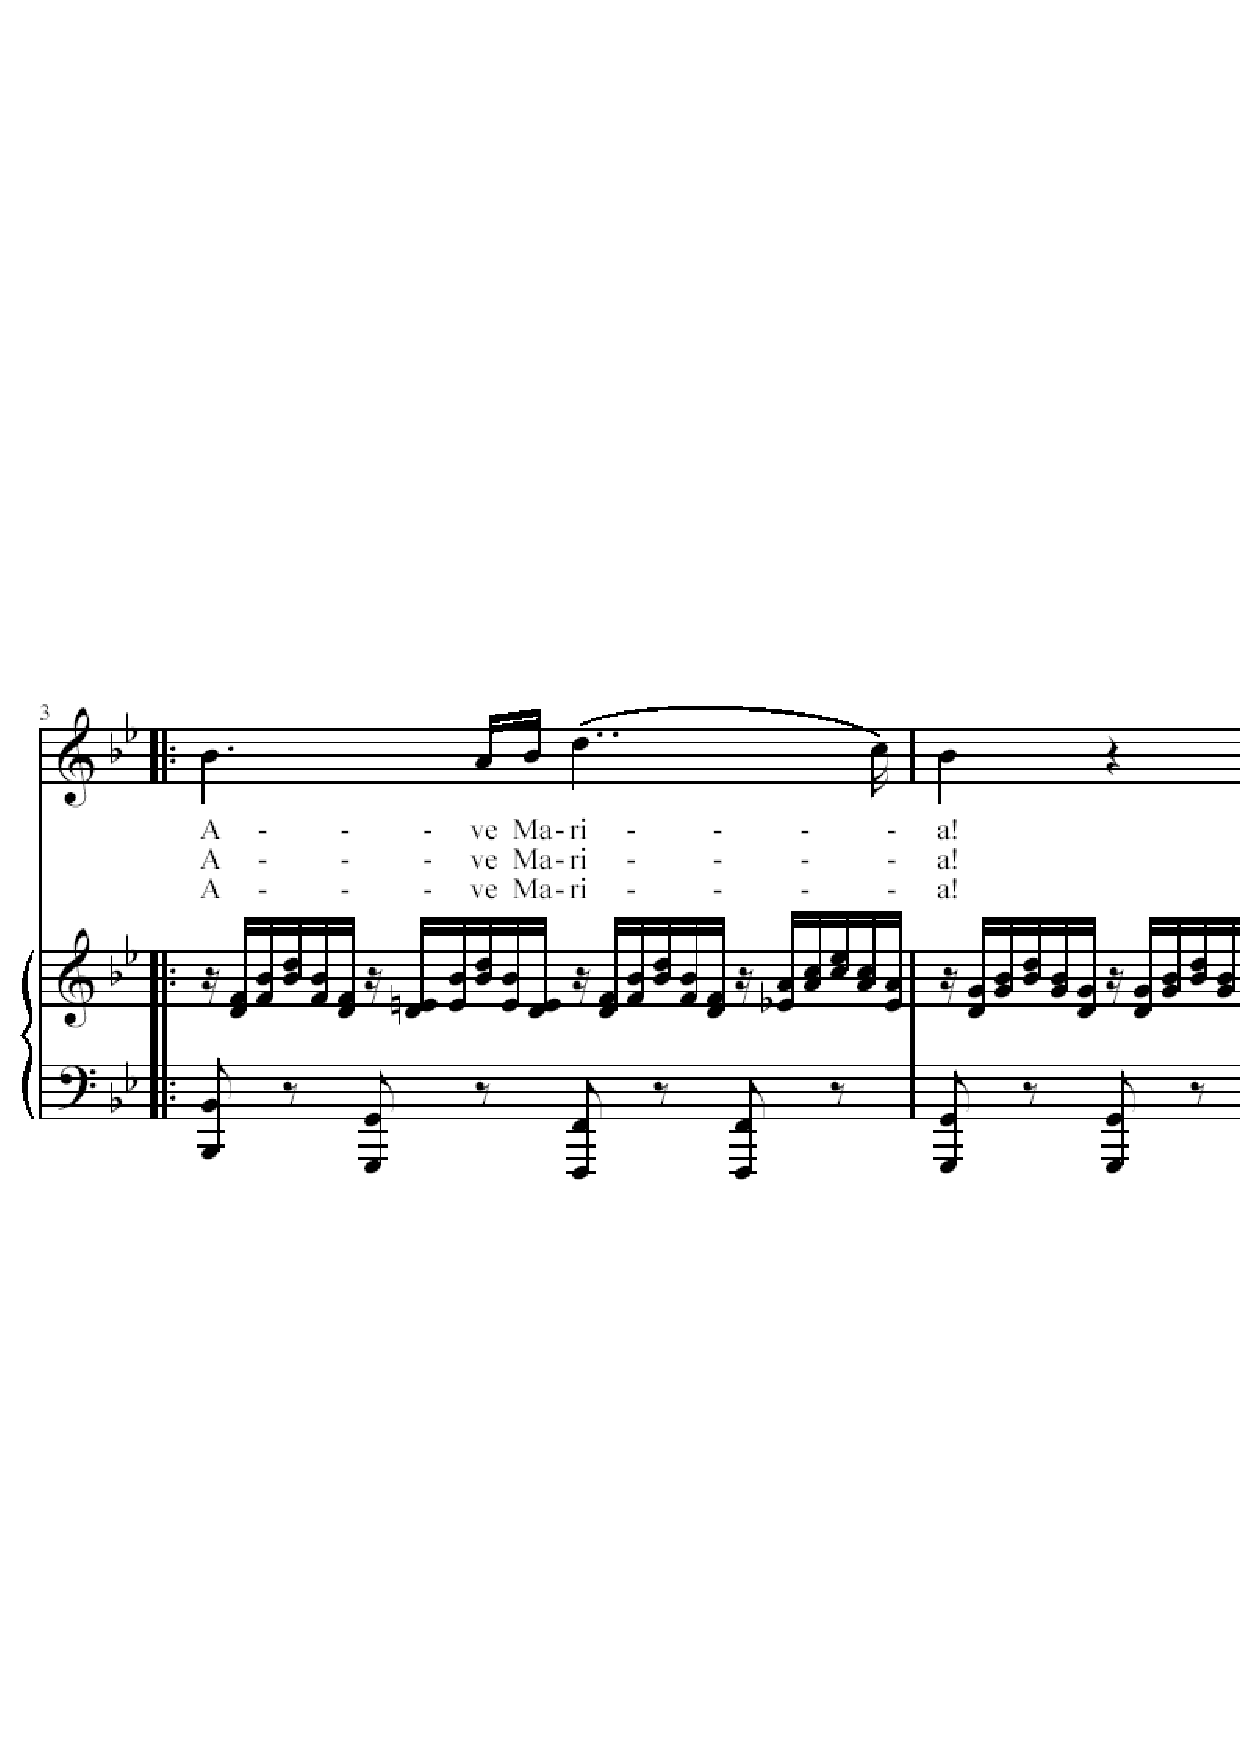
\includegraphics[scale=0.3,angle=-90]{graphics/music.pdf}
%        \caption{Musical Score of Franz Schubert's \emph{Ave Maria} (Ellen's Gesang III) \cite{musicxml}}
        \caption{Musical Score of Franz Schubert's \emph{Ave Maria} \cite{musicxml}}
        \label{music_figure}
    \end{center}
\end{figure}

The following knowledge templates deliver only short examples showing how music
may be modelled in CYBOL. Their property names were taken over from MusicXML's
element tags, as elaborated in \cite{musicxml}. Most are self-explanatory and
shall not be further discussed here. The first example template represents an
extract from a complete musical \emph{Work}, consisting of the two parts
\emph{Voice} and \emph{Piano}:

\begin{scriptsize}
    \begin{verbatim}
<model>
    <part name="number" channel="inline" abstraction="string" model="D. 839"/>
    <part name="title" channel="inline" abstraction="string" model="Ave Maria (Ellen's Gesang III)"/>
    <part name="composer" channel="inline" abstraction="string" model="Franz Schubert"/>
    <part name="poet" channel="inline" abstraction="string" model="Walter Scott"/>
    <part name="voice" channel="file" abstraction="cybol" model="voice.cybol">
        <property name="score_instrument" channel="inline" abstraction="string" model="P1-I14"/>
        <property name="instrument_name" channel="inline" abstraction="string" model="Choir Aahs"/>
        <property name="midi_instrument" channel="inline" abstraction="string" model="P1-I14"/>
        <property name="midi-channel" channel="inline" abstraction="integer" model="1"/>
        <property name="midi-program" channel="inline" abstraction="integer" model="53"/>
    </part>
    <part name="piano" channel="file" abstraction="cybol" model="piano.cybol">
        <property ...
    </part>
</model>
    \end{verbatim}
\end{scriptsize}

One of the \emph{Parts} is shown in the next template. It consists of several measures:

\begin{scriptsize}
    \begin{verbatim}
<model>
    <part name="measure_$1" channel="file" abstraction="cybol" model="measure_1.cybol">
        <property name="divisions" channel="inline" abstraction="integer" model="48"/>
        <property name="key_fifths" channel="inline" abstraction="integer" model="-2"/>
        <property name="key_mode" channel="inline" abstraction="string" model="major"/>
        <property name="beats" channel="inline" abstraction="integer" model="4"/>
        <property name="beat_type" channel="inline" abstraction="integer" model="4"/>
        <property name="staves" channel="inline" abstraction="integer" model="0"/>
        <property name="clef_sign" channel="inline" abstraction="string" model="G"/>
        <property name="clef_line" channel="inline" abstraction="integer" model="2"/>
    </part>
    <part name="measure_$2" channel="file" abstraction="cybol" model="measure_2.cybol">
        <property ...
    </part>
</model>
    \end{verbatim}
\end{scriptsize}

A \emph{Measure} again consists of \emph{Notes}:

\begin{scriptsize}
    \begin{verbatim}
<model>
    <part name="note_$1" channel="file" abstraction="cybol" model="note_1.cybol">
        <property name="duration" channel="inline" abstraction="integer" model="72"/>
        <property name="voice" channel="inline" abstraction="integer" model="1"/>
        <property name="type" channel="inline" abstraction="string" model="quarter"/>
        <property name="stem" channel="inline" abstraction="string" model="down"/>
        <property name="position" channel="inline" abstraction="integer" model="1"/>
    </part>
    <part name="note_$2" channel="file" abstraction="cybol" model="note_2.cybol">
        <property name="duration" channel="inline" abstraction="integer" model="12"/>
        <property name="voice" channel="inline" abstraction="integer" model="1"/>
        <property name="type" channel="inline" abstraction="string" model="16th"/>
        <property name="stem" channel="inline" abstraction="string" model="up"/>
        <property name="position" channel="inline" abstraction="integer" model="2"/>
    </part>
    <part name="note_$3" channel="file" abstraction="cybol" model="note_3.cybol">
        <property ...
        <property name="position" channel="inline" abstraction="integer" model="2"/>
    </part>
</model>
    \end{verbatim}
\end{scriptsize}

An important property to note here is the \emph{position} value. It is common
that two notes have to be played at the same time, the notes then being called
a \emph{Chord}. In contrast to MusicXML which provides an own tag to denote
notes belonging to the same chord, CYBOL suggests to use a \emph{position}
property having identical values for all notes in a chord. An interpreter
program may thus not only read necessary sequence information, but can also
figure out which of the notes have to be played \emph{synchronously}.

A fourth example represents one \emph{Note}, consisting of a \emph{Pitch} and
\emph{Lyric} text, which are the final abstractions in this knowledge template:

\begin{scriptsize}
    \begin{verbatim}
<model>
    <part name="pitch" channel="inline" abstraction="string" model="B">
        <property name="alter" channel="inline" abstraction="integer" model="-1"/>
        <property name="octave" channel="inline" abstraction="integer" model="4"/>
    </part>
    <part name="lyric" channel="inline" abstraction="string" model="A">
        <property name="syllabic" channel="inline" abstraction="string" model="begin"/>
    </part>
</model>
    \end{verbatim}
\end{scriptsize}
